\chapter{Results}
\label{cha:Results}
The simulator was designed to allow for variance in merge angle, lead in distances, speed limits, and traffic levels. This means that we can experiment to see what effect each of these variables has on the effectiveness of the QMM protocol. We can also compare the QMM protocol to the AIM protocol, using the modified version of the AIM simulator described in Section \ref{sec:Merge Schemes}.

\section{Experimental Procedure}
\label{sec:Experimental Procedure}
All experiments were done using pre-generated spawn schedules. In each experiment I used 20 pairs of schedules (1 schedule per lane). Schedule pairs are identical for tests with the same speed limit and traffic rate. Vehicles spawned for 1000 simulated seconds, and all vehicles were allowed to complete. The spawn schedules would only fail to spawn a vehicle if the spawning area was occupied by another vehicle. This caused reduced numbers of completed vehicles if the system became congested enough to cause queues up to the spawning area. 

\section{Comparing AIM and Queue Protocols}
\label{sec:Comparing AIM and Queue Protocols}
By using the modified AIM simulator described in section \ref{sec:Merge Schemes}, I obtained approximations for how well an AMM implementation would handle merges.

The AIM simulator has a lead in and lead out distance for each lane of 150 metres and is limited to 90\degree merges. These settings were duplicated for QMM. All of the lanes were set to have a speed limit of 20$\si{ms^{-1}}$ (44.7\si{mph} or 72\si{kph}). The traffic rate (vehicles/hour/lane (\si{vhl})) was altered to see how well the systems adjust to increasing levels of traffic.

In terms of reducing mean delay, both systems performed well at low traffic rates. From 500 to 1500\si{vhl} both systems kept mean delay below 2 seconds. AIM performed slightly better, hitting a mean delay 0.97\si{s} with a standard deviation of 1.35\si{s}, QMM achieved a mean delay of 1.84\si{s} with a standard deviation of 2.22\si{s}. As the traffic rates increased however, the performance of QMM degraded massively in comparison to AIM. At 2500\si{vhl} QMM hit a mean delay of 45.78\si{s} with a standard deviation of 18.13\si{s}. In comparison, AIM hit a mean delay of 5.43\si{s} and a standard deviation of 6.25\si{s}. Even with a high standard deviation like this, it's clear that AIM outperforms QMM in this respect. Figure \ref{fig:meanDelayTrafficRate} shows how the average delay increases over time for both systems.

\begin{figure}[htb]
\includegraphics[width=\textwidth]{plots/trafficRate/meanDelay.png}
\caption{Plot showing mean delay/traffic rate performance by merge management system.}
\label{fig:meanDelayTrafficRate}
\end{figure}

In terms of balancing mean delay over both lanes, QMM also fails to perform as well as AIM. At 500\si{vhl} the mean target lane delay for QMM is 0.06\si{s}, with a standard deviation of 0.25\si{s}. For the merge lane, the delay is 1.36\si{s}, with a standard deviation of 0.95\si{s}. Comparatively AIM has a mean delay of 0.37\si{s}, with a standard deviation of 0.79\si{s}, for the target lane, and 0.16\si{s}, with a standard deviation of 0.47\si{s}, for the merge lane.

At higher traffic rates the gap between the AIM lanes increases. At 2500\si{vhl} AIM has a mean delay of 1.75\si{s}, with a standard deviation of 1.54\si{s}, for the target lane, and 9.11\si{s}, with a standard deviation of 6.79\si{s}, for the merge lane. These times are still far better than the mean delays in QMM. Figure \ref{fig:meanDelayByLaneTrafficRate} shows the delay for each lane under each system.

\begin{figure}[htb]
\centerline{
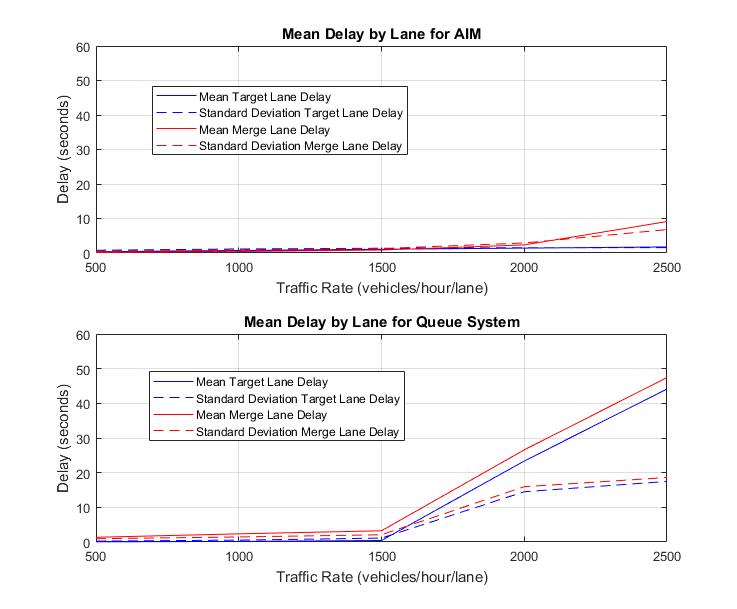
\includegraphics[width=15cm]{plots/trafficRate/meanDelayByLane.png}
}
\caption{Plots showing mean delay by lane for both merge management systems}
\label{fig:meanDelayByLaneTrafficRate}
\end{figure}

Both systems manage to maintain similar throughputs until the traffic rate increases past 1500\si{vhl}. By 2500\si{vhl}, AIM can deal with an extra 366 vehicles per hour compared to QMM. Figure \ref{fig:throughputTrafficRate} shows the throughputs for each system.

\begin{figure}[htb]
\centering
\includegraphics[width=10.5cm]{plots/trafficRate/throughput.png}
\caption{Plot showing throughput for both merge management systems}
\label{fig:throughputTrafficRate}
\end{figure}

These trends clearly demonstrate that AIM performs far more effectively at high traffic rates than QMM. AIM makes better use of space-time, so when the roads begin getting more congested, this pays off in AIMs favour. QMM ends up causing problems at these high traffic rates as it only allows one vehicle into the merge zone at any one time. QMM would work well for controlling roads with lower traffic rates, however, if the roads are expected to deal with congestion or high volume fast flowing traffic, the AIM system becomes the only viable option.

This test makes a good case for continuing attempts to develop an AMM system. This system would need to be able to work for other merge angles, as no research was conducted into the effectiveness of AIM at shallower angles. Further development would also need to done using a simulator which deals with some of the implementation problems found in the AIM simulator. As detailed in section \ref{sec:Simulation}, collisions and early arrival times were constant problems with attempts to implement an AMM system in the AIM simulator.

\section{The Effect of the Merge Angle}
\label{sec:The Effect of the Merge Angle}
The merge angle affects both the length of the merge zone and the angle at which vehicles join the target lane. For QMM to be effective, it should be able to deal with a range of merge angles.

For each test, the speed limit for both lanes was 20$\si{ms^{-1}}$ (44.7\si{mph} or 72\si{kph}) and each lane had a lead in distance of 150\si{m}. The traffic rate was set to 1000\si{vhl}.

At shallow angles QMM performed very poorly. Figure \ref{fig:meanDelayMergeAngle} shows how the shallow angle performance compares to steeper angles. At the shallowest angle tested, 5\degree, the system had a mean delay of 138.98\si{s} with a standard deviation of 46.96\si{s}. After the merge angle increases to around 30\degree, performance has improves greatly with the mean delay reaching 13.12\si{s} with a standard deviation of 9.35\si{s}. By the time the merge zone has reached it's minimum length, the mean delay has decreased to 1.24\si{s} with a standard deviation of 1.55\si{s}. The delay is actually smaller at 85\degree at 1.23\si{s} but this is well within range of the standard deviation for 90\degree. The delay of both the target lane and merge lane follow very similar trends. 

\begin{figure}[htb]
\centering
\includegraphics[width=10.0cm]{plots/mergeAngle/meanDelay.png}
\caption{Plot showing mean delay by merge angle}
\label{fig:meanDelayMergeAngle}
\end{figure}

In general throughput increases dramatically with the merge angle until around 35\degree where levels off dramatically. The data does show a dip in the merge lane throughput measurements from 40\degree to 60\degree. Investigation showed that this was an error with vehicle spawn system which dropped vehicles after detecting that there was still another vehicle in the spawn area. These were false detections due to the change in angle. A solution to the problem would have required separate spawn schedules for each angle which reduces the validity of the results. These results are considered to be outliers. Figure \ref{fig:throughputMergeAngle} shows how the throughput improves as the angle increases.

\begin{figure}[htb]
\centering
\includegraphics[width=10.0cm]{plots/mergeAngle/throughput.png}
\caption{Plot showing throughput by merge angle}
\label{fig:throughputMergeAngle}
\end{figure}

Shallow merge angles have such a drastic effect on performance because as the merge angle becomes shallower the merge zone gets longer. This means that the space time inefficiency of QMM has a huge effect on performance as vehicles have to wait for longer before they can enter the merge. One approach for dealing with shallow merges is to introduce a slip road instead of a merge zone. This would require a different system, as queuing wouldn't be appropriate in that situation.

\section{The Effect of Lead in Distances}
\label{sec:The Effect of Lead in Distances}
The lead in distance had very little effect on the overall success of the simulation. Below 100\si{m} there was some increase in delay due to the 150\si{m} distance limit before vehicles are added to the queue. Appendix \ref{sec:Lead in Distance Analysis} discusses these results in more detail.

\section{The Effect of Differing Speed Limits}
\label{sec:The Effect of Differing Speed Limits}
The speed limits of each lane and their differences impact how well a vehicle can move into another lane and adjust to its velocity. Many merges will be movements from lanes of differing speed, so its important that the queue system can handles these merges.

The traffic rate was set to 1000\si{vhl}, the merge angle was 45\degree, and the lead in distances were both set to 150\si{m}. Pairs of speeds were compared. The speed limits used were 10$\si{ms^{-1}}$, 20$\si{ms^{-1}}$, 30$\si{ms^{-1}}$, and 40$\si{ms^{-1}}$ (22.4\si{mph}, 44.7\si{mph}, 67.1\si{mph}, and 89.5\si{mph} or 36\si{kph}, 72\si{kph}, 108\si{kph}, and 144\si{kph} respectively). These speeds, excluding 40$\si{ms^{-1}}$, are very close to realistic speed limits and should provide insight into the real world applicability of the system.

The target lane suffers the most interference from the merge lane whenever the target lane's speed limit is larger than the merge lane's speed limit. This can be seen well in the relationship between a target lane speed limit of 30$\si{ms^{-1}}$ and a merge lane speed limit of 10$\si{ms^{-1}}$. The mean delay on the target lane is 13.92\si{s} with a standard deviation of 3.56\si{s}. Comparatively the merge lane had a mean delay of 4.01\si{s} with a standard deviation of 2.87\si{s}. 

Switching the lane speeds shows that the merge lane also experiences larger delays when the merge lane speed limit is larger than the target lane. When the target lane has a speed limit of 10$\si{ms^{-1}}$ and the merge lane has a speed limit of 30$\si{ms^{-1}}$, the merge lane has a mean delay of 12.00\si{s} with a standard deviation of 3.00\si{s}. In this case the target lane has a mean delay of 0.34\si{s} with a standard deviation of 0.95\si{s}.

It should be noted that when the speed gaps are smaller the effect on the lanes is reduced. Most of the speed limits containing a 40$\si{ms^{-1}}$ lane also performed poorly. The velocity causes vehicles to accumulate too quickly for the queue system to be able to sort them out effectively. Figure \ref{fig:meanDelaySpeedLimit} shows how the mean delay is affected by difference speed limit pairs.

The number of vehicles that complete for each lane is solely affected by the speed limit of the lane, the differences between the lanes has very little effect. The throughput is likewise only affected by the speed limits of each lane independently. Figure \ref{fig:throughputSpeedLimit} shows how the throughput is affected by the speed limits.

\begin{figure}[htb]
\includegraphics[width=\textwidth]{plots/speedLimit/throughput.png}
\caption{Bar chart showing throughput by speed limit pair}
\label{fig:throughputSpeedLimit}
\end{figure}

\begin{figure}[p]
\centerline{
	\includegraphics[height=\textheight]{plots/speedLimit/meanDelay.png}
}
\caption{Bar chart showing mean delay by speed limit pair}
\label{fig:meanDelaySpeedLimit}
\end{figure}

These results show that QMM struggles to handle differences in velocity well, with the faster lane being impacted more heavily than the slower lane. This is because the faster lane is forced to slow down to accommodate the slower lane. There will always be delay on the faster lane due to this reason. The aim for a good merge system is to minimise the effect of the speed limit gap as much as possible.


